\section{Zugqualität}
Mit der Zugqualität möchten wir herausfinden, welche Evaluationsfunktion bzw. welche Kombination von Evaluationsfunktionen \enquote{am besten} ist.
Um \enquote{das Beste} zu definieren, verwenden wir Stockfish 18 als Referenzengine. Stockfish 18 ist die neuste Version von Stockfish (Stand: März 2026). \\
Stockfish wurde gewählt, da es derzeit als führender Schachcomputer angesehen werden kann (siehe \ref{subsec:vergleichSchachcomputer}).

\subsection{Testaufbau}

Zunächst wurde mit einer KI Kategorien und Positionen generiert. Diese wurden anschliessend überprüft und
kritisch hinterfragt. Daraus ergaben sich 20 Positionen, die in 4 Kategorien unterteilt wurden:
Taktik, dynamisches Spiel, Positionsspiel und Endspiel.

Beim Test wird für jede Position mit jeder möglichen Evaluationsfunktion bzw. Evaluationsfunktionskombination (mit Ausnahme von
MateAwareEval allein) der beste Zug mit einer Tiefe von 8 berechnet.
Stockfish rechnet ebenfalls bis zur Tiefe 8. Zusätzlich berechnet er auch 5 bestmöglichen Züge. Dies kann mit dem Befehl \textit{MultiPV}
erreicht werden (\cite{stockfishMultiPv}).

Anschliessend wird verglichen, ob eine unserer Evaluationsfunktionen den besten, zweitbesten oder allgemein einen der
von Stockfish ermittelten Top-Züge findet. Auf Grundlage eines Punktesystems werden dafür unterschiedlich viele Punkte
vergeben: Für den besten Zug werden 8 Punkte vergeben, für den zweitbesten 6 usw.:

\lstinputlisting[
    firstline=113,
    lastline=113,
    firstnumber=1,
    caption={QualityTest - Verteilung der möglichen Punkte},
    label={lst:qualitTestHeadPointDistro}
]{../src/test/java/ch/hslu/cas/msed/blobfish/QualityTest.java}

Anhand der erreichten Punktzahl und der gewählten Züge können die Evaluationsfunktionen nun miteinander verglichen werden.

\subsubsection{Learnings aus einer vorherigen Ausführung}

Derselbe Test wurde schon mit einer Tiefe von 5 ausgeführt. Bei der Analyse der Testresultate wurde bemerkt, dass eine
gerade Zahl als Tiefe gewählt werden muss, um sicherzustellen, dass der nächstmögliche Zug vom Gegner ebenfalls
berücksichtigt wird. Ansonsten werden werden viele \enquote{unsinnige} Züge vorgeschlagen. Ebenfalls wurde entschieden
eine noch höhere Zahl gewählt, in der Hoffnung, ein noch besseres Ergebnis erziehlen zu können.

MateAwareEval alleine wurde ebenfalls nicht mehr berücksichtig, was als learning von einer vorherigen Testsausführung ist:
Die Funktion MateAwareEval stellt nur sicher, dass Züge, welche zum Schachmatt führen, gewinnen. Falls jedoch dies
nicht direkt ausgeführt werden kann, bringt diese Evaluation nichts und unsere es wird der ersten berechneten
Schachzug vorgeschlagen, was zufälligerweise ein guter oder schlechter Zug sein kann. Um diese Zufälligkeit aus unsere Analyse
zu entfernen, haben wir uns entschieden, diese Evaluation alleinstehend nicht mehr zu beurteilen.

\subsection{Testresultate}

Nachfolgend werden pro Kategorie die Testresultate dargestellt. In den Diagrammen sind
jedoch nicht mehr die einzelnen Züge und deren Ergebnisse zu sehen. Diese sind im Anhang unter \ref{zugqualit_tabel} zu finden.

\begin{figure}[H]
    \centering
    
\includegraphics[width=\linewidth]{evaluation/report/movequality/DynamicPlayInitiativeSacrifices}
    \caption{Testresultat Zugqualität - Dynamic play / initiative / sacrifices}
    \label{fig:resultatZugQualityDynamicPlay}
\end{figure}

\begin{figure}[H]
    \centering
    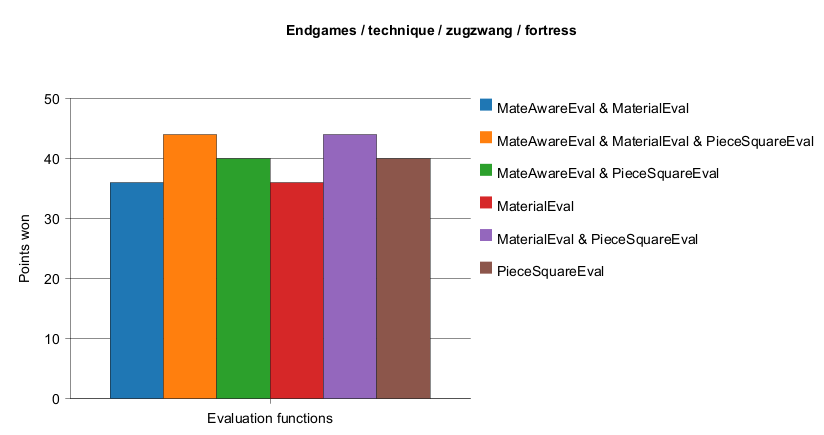
\includegraphics[width=\linewidth]{evaluation/report/movequality/EndgamesTechniqueZugzwangFortress}
    \caption{Testresultat Zugqualität - Endgames / technique / zugzwang / fortress}
    \label{fig:resultatZugEndgame}
\end{figure}


\begin{figure}[H]
    \centering
    
\includegraphics[width=\linewidth]{evaluation/report/movequality/PositionalPlayProphylaxis}
    \caption{Testresultat Zugqualität - Positional play / prophylaxis}
    \label{fig:resultatZugQualityPositonalPlay}
\end{figure}


\begin{figure}[H]
    \centering
    
\includegraphics[width=\linewidth]{evaluation/report/movequality/Tactics}
    \caption{Testresultat Zugqualität - Tactics}
    \label{fig:resultatZugQualityTactics}
\end{figure}

*Hier hinzufügen wie die overall rechnung ist*

\subsection{Intepretation}

Wie zu erwarten hat die Evaluation gewonnen, welche am meisten berücksichtigt. Hierfür spricht, dass es eine gute
Balance zwischen den Evaluationen gibt und die richtige gewinnt. \\
Spannend ist, wie

